\documentclass[conference]{IEEEtran}

\usepackage[utf8]{inputenc}
\usepackage[T1]{fontenc}
\usepackage{cite}
\usepackage{amsmath,amssymb,amsfonts}
\usepackage{algorithmic}
\usepackage{graphicx}
\usepackage{textcomp}
\usepackage{xcolor}
\usepackage{booktabs}
\usepackage{hyperref}
\usepackage{microtype}

\graphicspath{{../datasheet/figures/}{../../../../lib/prra/images/}}

\begin{document}

\title{HyNoC: A Hybrid Circuit-Switch/Wormhole\\
Network-on-Chip for Distributed VLIW\\
Computing on FPGA}

\author{
  \IEEEauthorblockN{Christophe Clienti}
  \IEEEauthorblockA{%
    \textit{Open Hardware Project}\\
    CERN-OHL-P v2.0\\
    \href{https://github.com/cclienti/verilog-ip}{https://github.com/cclienti/verilog-ip}}
}

\maketitle

\begin{abstract}
Network-on-Chip (NoC) architectures have become the standard interconnect fabric
for many-core systems, yet most proposals face a fundamental trade-off between
latency, area, and congestion management. This paper presents \textbf{HyNoC}
(Hybrid Network-on-Chip), an open-source NoC architecture that combines
circuit-switch path establishment with wormhole data transfer, targeting
distributed computing systems built around VLIW processor cores on FPGA.

HyNoC employs source routing, where the complete path through the network is
encoded in the packet header by the sender or statically at compile time, enabling
both deterministic low-latency transfers and software-level hotspot avoidance
without the area overhead of virtual channels. The router features a parallel
round-robin arbiter (PRRA) with fixed grant latency, per-port independent clock
domains, and support for both unicast and multicast routing.

We discuss the design rationale, the hybrid switching model, and positioning
relative to prior NoC art, and argue that a richer topology combined with
compiler-assisted static routing is a competitive alternative to virtual channels
for FPGA-based distributed VLIW systems. The complete RTL implementation is
released as open-source hardware under the CERN-OHL-P~v2 license. The Veriparse source-to-source elaboration toolkit~cite{veriparse} is provided as a companion tool to handle advanced RTL constructs and accelerate simulation.
\end{abstract}

\begin{IEEEkeywords}
Network-on-Chip, FPGA, source routing, wormhole switching, circuit switching,
VLIW, parallel round-robin arbiter, open-source hardware.
\end{IEEEkeywords}

\section{Introduction}
\label{sec:introduction}

As the number of processing elements integrated on a single chip increases,
scalable on-chip communication becomes a first-class design concern.
Network-on-Chip (NoC) architectures have emerged as the standard answer to this
challenge, replacing shared buses and point-to-point links with a structured,
packet-switched interconnect fabric~\cite{dally2001}.

Existing NoC designs span a broad design space. Wormhole switching minimizes
buffering by forwarding flits as soon as the header is decoded, but exposes the
network to head-of-line blocking. Virtual channels (VCs) were introduced to
mitigate this blocking~\cite{dally1992}, at the cost of duplicated buffers that
can represent the dominant area contribution of a router~\cite{mello2005}. Circuit
switching provides fully dedicated, contention-free paths but requires path
reservation before any data can flow.

\textbf{HyNoC} takes a different approach: it combines the path-dedication
property of circuit switching---through a source-routed request/grant handshake at
each hop---with the flit-level, FIFO-backed flow control of wormhole switching.
This hybrid model is particularly well suited to FPGA targets, where block RAMs
used as FIFOs are scarce resources, and to distributed VLIW computing workloads,
where communication patterns are largely known at compile time and can therefore be
routed statically to avoid congestion.

Originally inspired by the Hermes NoC~\cite{moraes2004}, HyNoC departs
significantly from its ancestor by introducing distributed arbitration, relative
source routing with multicast support, per-port asynchronous clock domains, and a
parallel round-robin arbiter that grants requests in a one or two cycles.

The contributions of this paper are:
\begin{itemize}
  \item A precise characterization of HyNoC's hybrid switching model and its
        implications for latency and area;
  \item A discussion of static route management as an alternative to virtual
        channels, supported by a combinatorial analysis of shortest-path counts
        in mesh and higher-dimensional topologies;
  \item An analysis of the scope and limitations of the no-VC design choice;
  \item An open-source RTL implementation targeting both simulation and FPGA
        synthesis, complemented by the Veriparse toolkit~\cite{veriparse} for
        source-to-source elaboration of advanced RTL constructs and faster
        simulation;
  \item Verilator co-simulation results measuring the deterministic, linear
        per-hop latency and demonstrating link-disjoint quadrant isolation under
        a LLaMA~3~8B-scale distributed GeMV workload.
\end{itemize}

The remainder of the paper is organized as follows.
Section~\ref{sec:related} reviews related work.
Section~\ref{sec:architecture} describes the HyNoC architecture.
Section~\ref{sec:switching} details the hybrid switching model and the rationale
for avoiding virtual channels.
Section~\ref{sec:target} discusses the target application domain.
Section~\ref{sec:implementation} presents implementation details.
Section~\ref{sec:evaluation} reports simulation results, and
Section~\ref{sec:conclusion} concludes.

\section{Related Work}
\label{sec:related}

\subsection{Switching Strategies}

Three main switching strategies are found in the NoC literature.
\emph{Store-and-forward} switching requires a complete packet to be buffered at
each router before forwarding, providing clean error isolation but imposing large
buffer requirements and high latency~\cite{dally2001}.
\emph{Wormhole switching}~\cite{dally1987} pipelines flits across routers,
dramatically reducing buffer depth requirements; latency depends on path length
and contention.
\emph{Circuit switching}~\cite{kumar2002} reserves a dedicated path before
transmission, eliminating mid-network contention at the cost of reservation
overhead.

Hybrid approaches have been explored. Æthereal~\cite{goossens2005} combines
guaranteed-throughput circuit-switched slots with best-effort wormhole traffic on
the same physical links. HyNoC differs: it uses source routing to establish a
dedicated path through a series of request/grant handshakes (the circuit phase),
then streams flits in wormhole fashion along that path (the data phase), with no
time-division multiplexing.

\subsection{Routing Algorithms}

XY deterministic routing~\cite{dally2001} is simple and deadlock-free on 2D
meshes but provides only a single path between any pair of nodes. Adaptive
routing~\cite{duato1993} improves load balancing but requires more complex router
logic and typically needs virtual channels to avoid deadlock.

\emph{Source routing} encodes the complete route in the packet header at the
sender. This approach, studied for NoCs in~\cite{liwei2007} and~\cite{mubeen2010},
shifts routing complexity from the router to the sending node or to an offline
compilation step. The router itself becomes simpler: it only needs to decode the
next hop from the current flit, forward it, and update the index. Source routing
naturally supports any topology without per-router routing table storage, and
allows the sender to choose among multiple paths.

HyNoC adopts source routing with a compact \emph{relative} hop encoding: since a
packet cannot exit from the same port it entered, a router with $P$ ports offers
only $P-1$ egress choices, encoded in $\lceil\log_2(P-1)\rceil$ bits per hop.
This reduces both header overhead and crossbar complexity simultaneously.

\subsection{Virtual Channels}

Virtual channels (VCs), introduced by Dally~\cite{dally1992}, multiplex several
logical channels over a single physical link, providing additional routing paths
and breaking deadlock cycles. Their main drawback is area: each VC requires a
dedicated buffer, and~\cite{mello2005} shows that router area scales nearly
linearly with VC count. On FPGAs, where block RAMs are shared between the
application and the communication infrastructure, this overhead is particularly
significant.

Several works have explored VC reduction or elimination.
Turn-model routing~\cite{glass1992} achieves deadlock freedom without VCs by
restricting turns in the routing graph. HyNoC's approach---providing path diversity
through richer topologies and compile-time route selection---aligns with this
trend, and is analyzed quantitatively in Section~\ref{sec:switching}.

\subsection{NoC Arbitration}

Round-robin arbiters are widely used for their fairness guarantees. Sequential
round-robin FSMs scan requests cyclically, introducing latency proportional to the
number of ports. HyNoC implements a \emph{parallel round-robin arbiter} (PRRA)
that combines the fairness of round-robin with a low-latency response: the arbiter
transitions directly to the state of any pending request, respecting a rotating
priority order, and responds in one or two cycles regardless of the number of
ports. The implementation relies on a LUT-mux structure that keeps the critical
path independent of port count.

\subsection{FPGA-Targeted NoCs}

Several NoC designs target FPGAs specifically. CONNECT~\cite{papamichael2012}
provides a parameterized, synthesizable NoC generator. HopliteRT~\cite{nair2019}
proposes a lightweight deflection-routing NoC without input buffers, achieving
extremely small area at the cost of non-deterministic latency. HyNoC targets a
different point: a fully parameterized, topology-agnostic NoC with bounded latency,
suited to predictable VLIW workloads.

\subsection{VLIW Many-Core Systems}

VLIW architectures expose instruction-level parallelism explicitly, making them
well suited for signal processing and scientific computing kernels~\cite{ellis1986}.
Distributed VLIW many-core systems---exemplified by the Kalray
MPPA~\cite{dinechin2013}---replicate simple VLIW cores connected through a NoC. In
such systems, communication patterns can be determined at compile time, making
static source routing particularly attractive.

\section{HyNoC Architecture}
\label{sec:architecture}

\subsection{Overview}

A HyNoC network is built by assembling routers with a configurable number of ports
(3 to 9 in the current implementation). Each router port is full-duplex, composed
of an ingress interface and an egress interface. Two neighboring routers are
connected by cross-linking their egress and ingress interfaces. Processing nodes
are attached through a \emph{local interface}, which adds an extra output FIFO to
decouple the node's clock domain from the router.

The router implements a \textbf{full crossbar}: any ingress port can simultaneously
communicate with any egress port, subject to arbitration. Multiple paths can be
open concurrently inside the same router, enabling full bisection bandwidth
utilization when traffic permits. Figure~\ref{fig:noc-overview} shows the internal
organization of 5-port routers and their interconnections.

\begin{figure}[t]
  \centering
  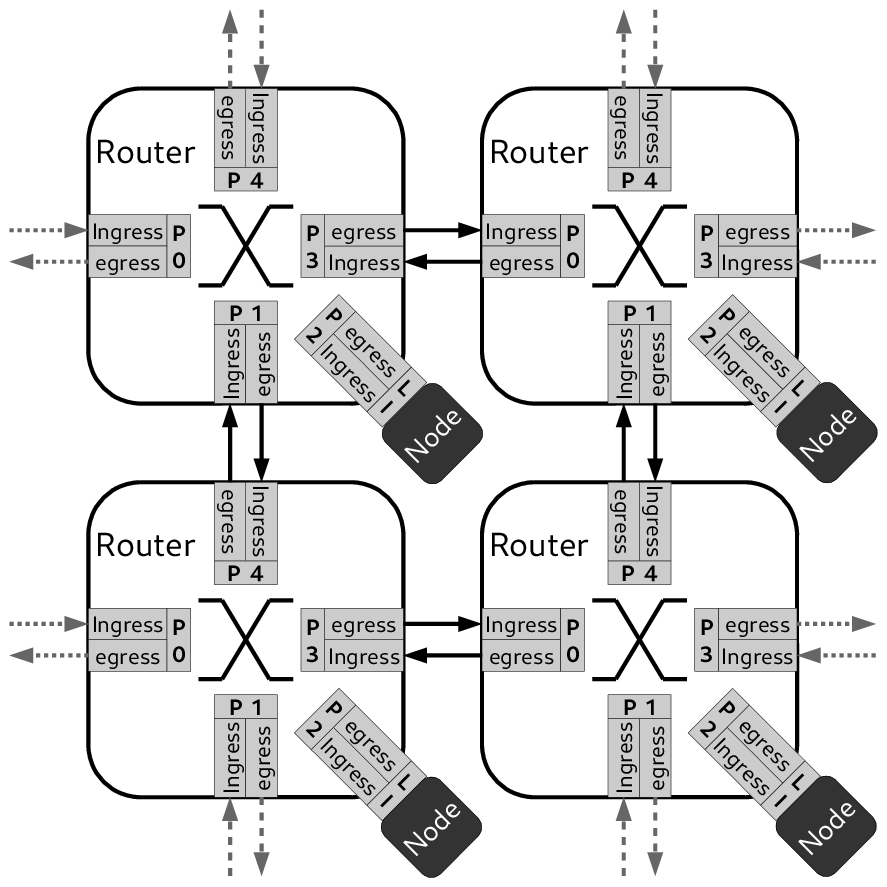
\includegraphics[width=\columnwidth]{hynoc_noc_overview}
  \caption{Router interconnections overview.}
  \label{fig:noc-overview}
\end{figure}

\subsection{Ingress Port}

The ingress port receives flits from the egress of a neighboring router. It buffers
incoming flits in a dual-clock FIFO (configurable depth: 2 to 64 entries), which
simultaneously handles clock domain crossing between the upstream router's clock
domain and the local router domain.

Once flits are available, the ingress FSM decodes the routing flit, extracts the
next-hop egress port identifier, and asserts a \emph{request} signal to the
corresponding egress port. It then waits for a \emph{grant}. Upon grant, the
ingress begins forwarding flits: if the routing flit still carries hops for
downstream routers (index $> 0$), it is updated (index decremented) and forwarded;
if the index has reached zero, the routing flit is consumed locally and not
forwarded. Subsequent payload flits are streamed directly to the granted egress
until the stop bit of the last flit is detected, at which point the channel is
released.

Flow control is managed by monitoring the FIFO level of the downstream router's
ingress FIFO. The ingress stalls when the downstream FIFO approaches full,
preventing flit loss. The internal data path of a 3-port router is illustrated in
Figure~\ref{fig:data-arch}.

\begin{figure}[t]
  \centering
  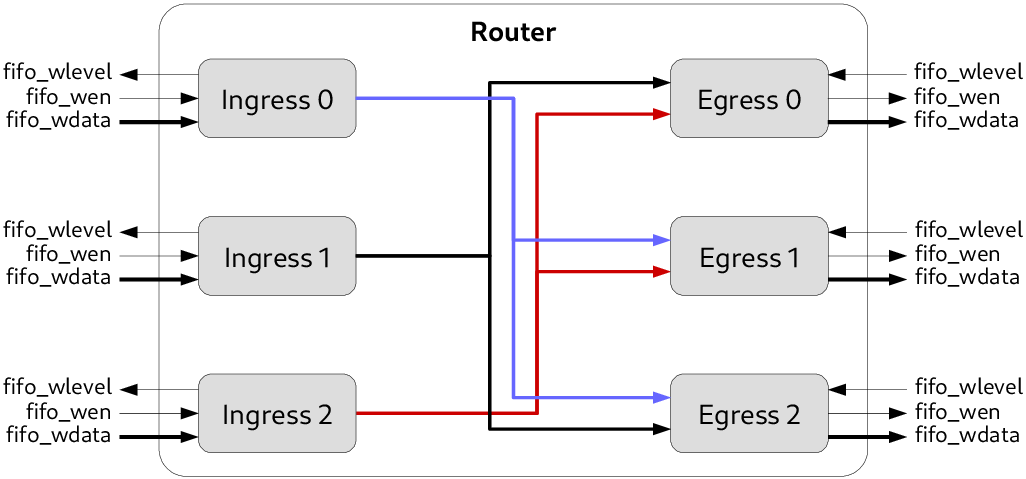
\includegraphics[width=\columnwidth]{hynoc_router_data_arch}
  \caption{Internal data path of a 3-port router.}
  \label{fig:data-arch}
\end{figure}

\subsection{Egress Port}

The egress port receives concurrent write requests from all $N-1$ ingress ports.
It arbitrates among them using the PRRA, grants one request at a time, and
connects the selected ingress data path to the downstream router's ingress FIFO.
The downstream FIFO level is forwarded back to the granted ingress for flow
control. The control path is shown in Figure~\ref{fig:ctrl-arch}: contrary to the
data path, control signals are point-to-point between each ingress and each egress,
avoiding broadcast of control information.

\begin{figure}[t]
  \centering
  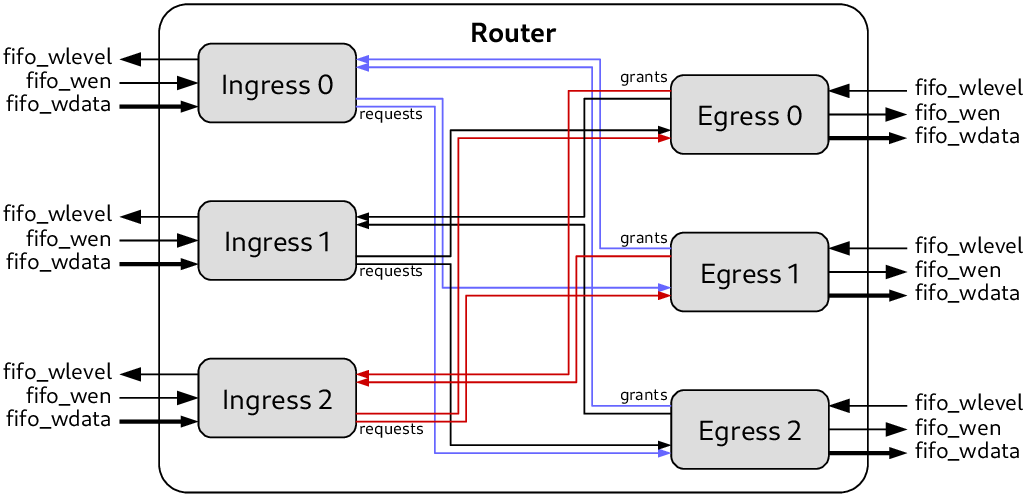
\includegraphics[width=\columnwidth]{hynoc_router_control_arch}
  \caption{Internal control path of a 3-port router.}
  \label{fig:ctrl-arch}
\end{figure}

\subsection{Parallel Round-Robin Arbiter (PRRA)}

The standard sequential round-robin FSM introduces up to $N$ cycles of latency
before granting a request. HyNoC replaces this with a \textbf{parallel
round-robin arbiter}: a LUT-based FSM that evaluates all pending requests
simultaneously, selects the highest-priority pending request according to a
rotating priority order, and transitions directly to the corresponding state.

The state transition $P_k$ is given by:
\begin{equation}
  P_k \leftarrow \text{request}[k] = 1
  \label{eq:prra}
\end{equation}
where $P_0$ carries the highest priority and $P_{N-2}$ the lowest. An additional
implicit transition keeps the current state while a granted request is active,
preventing spurious re-arbitration during packet transfer.

The arbiter responds in \textbf{one or two clock cycles} (configurable via the
\texttt{PRRA\_PIPELINE} parameter), regardless of the number of ports. The
critical path does not grow with $N$ because each state's transition equation is
stored in a dedicated LUT, selected by a multiplexer from the state register.
Starvation is prevented by the rotating priority: after serving request $k$,
priority rotates to port $k+1$.

\subsection{Clock Domain Architecture}

Each router port operates in its own clock domain. The dual-clock FIFO at each
ingress interface handles the crossing between the upstream port clock and the
local router clock. For timing-critical designs, a single-clock mode
(\texttt{SINGLE\_CLOCK\_ROUTER=1}) is available, reducing crossing latency.

The local interface adds an extra FIFO at the egress output, fully decoupling the
attached node's clock domain from the router.

\subsection{First Layer Protocol}

\subsubsection{Packet and Flit Structure}

The network operates on flits of $(\mathtt{PAYLOAD\_WIDTH}+1)$ bits. The most
significant bit is a \emph{stop bit}: when set, it marks the last flit of a
packet. A packet consists of one or more \emph{routing flits} followed by one or
more \emph{payload flits}. The routing flit carries a 4-bit \emph{Proto} field:

\begin{table}[h]
\centering
\caption{Supported routing protocols}
\label{tab:proto}
\begin{tabular}{@{}ll@{}}
\toprule
Proto & Routing method \\
\midrule
\texttt{4'b0000} & Unicast circuit switch \\
\texttt{4'b0001} & Multicast circuit switch \\
\texttt{4'b1000} & XY routing (reserved) \\
\texttt{4'b1111} & Forbidden \\
\bottomrule
\end{tabular}
\end{table}

\subsubsection{Unicast Source Routing}

The routing flit carries $H$ hop fields of $\lceil\log_2(P-1)\rceil$ bits each,
encoding the relative egress port ID at the next router. An \emph{index} field
(initialized to $H-1$) points to the hop to be consumed by the next router. The
ingress port decrements the index after consuming a hop; if the index was already
zero, the routing flit is not forwarded downstream. The relative hop encoding is
illustrated in Figure~\ref{fig:hops}.

\begin{figure}[t]
  \centering
  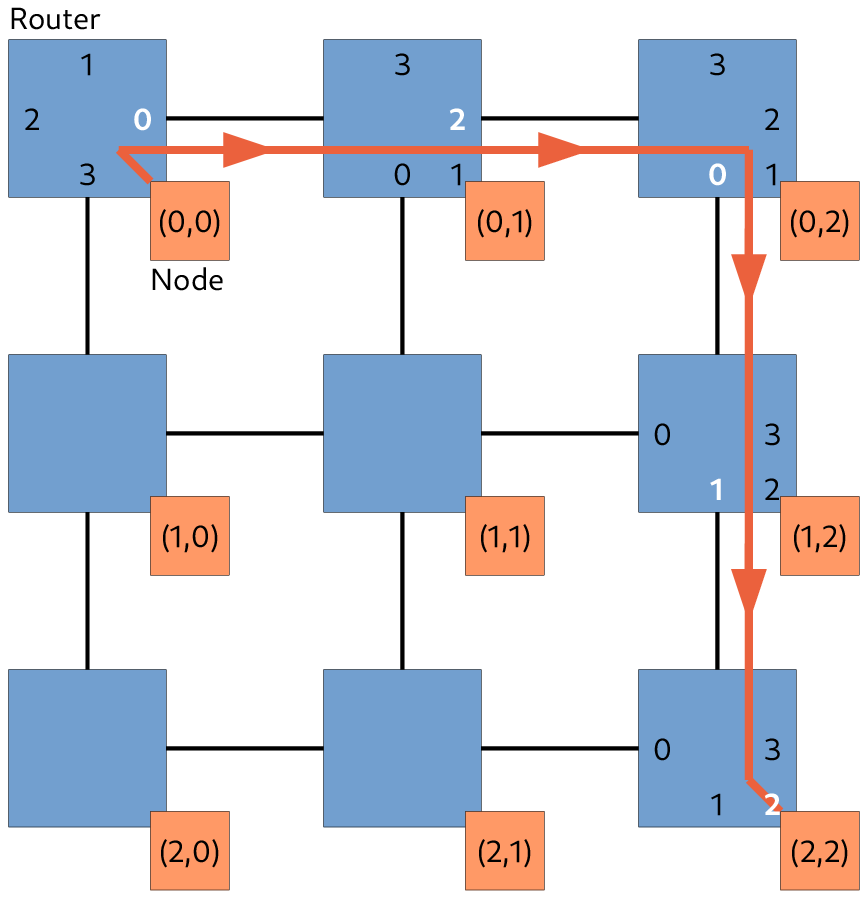
\includegraphics[width=0.85\columnwidth]{hynoc_hops_encoding}
  \caption{Relative hop encoding for a $3\times 3$ mesh network.}
  \label{fig:hops}
\end{figure}

The relative encoding (egress IDs numbered counterclockwise from the ingress port,
excluding that port) reduces both the hop field width and the internal crossbar
size.

\subsubsection{Multicast Source Routing}

In multicast mode, each hop field is a bitmask of width $P-1$, where each bit
selects one egress port. The packet is duplicated and forwarded to all asserted
egress ports simultaneously. Multiple routing flits with different multicast masks
can be chained to address complex multicast trees. This is particularly useful for
broadcast operations in VLIW many-core workloads.

\section{Hybrid Switching Model and Design Rationale}
\label{sec:switching}

\subsection{The Hybrid Switching Model}

HyNoC's switching model is best described as \emph{circuit-switched wormhole}: it
combines a \textbf{circuit-establishment phase} with a \textbf{wormhole data
phase}.

In the \textbf{circuit-establishment phase}, the ingress port asserts a request to
a specific egress port (identified from the routing flit) and waits for a grant.
This request/grant handshake propagates along the route: once the first router
grants the request, the ingress begins forwarding flits, which in turn trigger the
same handshake at the next router. A dedicated forwarding path through the network
is thus progressively opened, hop by hop.

In the \textbf{wormhole data phase}, payload flits are streamed flit-by-flit along
the established path, regulated by FIFO-level flow control. The path remains
dedicated to this packet until the stop bit is observed, ensuring in-order,
contention-free delivery once the channel is open.

This combination provides the \emph{low buffering} advantage of wormhole switching
(only the ingress FIFO is needed, no full packet storage) while offering the
\emph{path dedication} advantage of circuit switching (no mid-network arbitration
contention during payload transfer). The trade-off is a path-establishment latency
proportional to the route length before the first payload flit is delivered at the
destination.

\subsection{Static Route Management as an Alternative to Virtual Channels}

Virtual channels were introduced primarily to: (1) provide additional logical paths
to avoid deadlock; and (2) reduce head-of-line blocking under congestion. HyNoC
addresses both goals differently.

\textbf{Deadlock avoidance} is achieved through source routing itself: the
complete path is determined by the sender and can be constrained to acyclic
subgraphs (e.g., dimension-order routing) without any router-internal mechanism.

\textbf{Congestion avoidance} is addressed at two levels. First, the compiler or
runtime system assigns routes across multiple available shortest paths, distributing
traffic away from known hotspots. The number of shortest paths between two nodes in
an $N \times M$ mesh is a classical combinatorial result~\cite{knuth1997}: each path consists of a fixed sequence of moves along each dimension, taken in any order, and the count is given by the multinomial coefficient:

\begin{equation}
  p = \binom{(N-1)+(M-1)}{N-1} = \frac{[(N-1)+(M-1)]!}{(N-1)!\,(M-1)!}
  \label{eq:paths2d}
\end{equation}

This generalizes to a $K$-dimensional network $n_1 \times n_2 \times \cdots \times
n_K$ as:

\begin{equation}
  p = \frac{\left[\sum_{i=1}^{K}(n_i-1)\right]!}{\prod_{i=1}^{K}(n_i-1)!}
  \label{eq:pathsnd}
\end{equation}

Note that~(\ref{eq:paths2d}) and~(\ref{eq:pathsnd}) give the number of shortest
paths between the \emph{most distant} node pair (corner-to-corner). For an
arbitrary pair separated by $(d_x, d_y)$ hops the count is $\binom{d_x+d_y}{d_x}$,
which is lower. Table~\ref{tab:paths} reports corner-to-corner values for
representative 2D mesh topologies.

\begin{table}[h]
\centering
\caption{Shortest path counts in 2D mesh NoCs (corner-to-corner)}
\label{tab:paths}
\begin{tabular}{@{}lrrl@{}}
\toprule
Topology & Routers & Shortest paths & Path length \\
\midrule
$2\times 2$   &   4 &               2 &  2 \\
$4\times 4$   &  16 &              20 &  6 \\
$8\times 8$   &  64 &           3\,432 & 14 \\
$16\times 16$ & 256 & 155\,117\,520    & 30 \\
\bottomrule
\end{tabular}
\end{table}

Second, for applications with more dynamic traffic, the network topology can be
enriched with additional relay routers (without local interfaces), increasing path
diversity proportionally to the added area.

\subsection{Area Comparison with Virtual Channels}

Following~\cite{mello2005}, router area scales linearly with the number of VCs
(each VC requires an additional input buffer per port). An $8\times 8$ mesh with
4~VCs consumes the equivalent area of a $16\times 16$ mesh without VCs, yet the
latter offers 66$\times$ more shortest paths between corner nodes. On FPGA, where
block RAMs are scarce, minimizing buffer count is a primary concern.

The VC area model is itself optimistic in two respects: (1) the crossbar logic and
VC scheduler also grow with VC count; (2) VC path diversity is an upper bound,
since in practice the VC is assigned at the source and remains fixed for the entire
path, providing less diversity than a true additional physical dimension.
Conversely, the physical router area model does not capture link wiring cost, which
may be relevant in ASIC contexts.

\subsection{Head-of-Line Blocking and Mitigations}

Once a channel is granted, it remains dedicated until the stop bit of the last
flit is received. A long packet therefore delays other packets competing for the
same egress port. Two complementary mitigations are available in HyNoC:

\begin{enumerate}
  \item \textbf{Network enrichment}: adding more routers distributes traffic
    across more egress ports, reducing the probability that multiple flows compete
    for the same port. The cost is increased end-to-end \emph{latency} due to
    additional hops---this is the primary performance trade-off, not throughput.
  \item \textbf{Multiple local interfaces}: a node can expose several local
    interfaces connected to different router ports, providing as many independent
    logical channels as needed. This replicates the path diversity benefit of VCs
    without duplicating internal router buffers. It is the recommended approach
    when a node requires simultaneous, non-blocking communication with multiple
    peers.
\end{enumerate}

\subsection{Scope and Limitations}

The topology-based approach is most effective when traffic patterns are known at
compile time and routes can be assigned statically. When traffic is entirely
unpredictable at design time and topology enrichment is not feasible, virtual
channels remain the more appropriate solution. HyNoC targets systems---distributed
VLIW processors on FPGA---where compile-time route assignment is natural and FPGA
resource budgets make buffer minimization a primary concern.

\section{Target Application: Distributed VLIW Computing}
\label{sec:target}

\subsection{VLIW Cores and Compile-Time Scheduling}

VLIW processors expose multiple functional units to the compiler, which schedules
operations explicitly in long instruction words~\cite{ellis1986}. This design
philosophy shifts control complexity from hardware to software, resulting in
simple, area-efficient cores well suited for replication in many-core arrays.
Signal processing, scientific computing, and neural network inference kernels are
representative workloads.

In a distributed VLIW many-core system, each core executes a portion of a
data-flow graph, passing intermediate results to neighboring cores through the
NoC. The communication graph is typically known at compile time, enabling the
compiler to:
\begin{enumerate}
  \item Assign each communication a source route through the NoC;
  \item Schedule packet injections to avoid simultaneous contention on the same
        egress port;
  \item Guarantee bounded communication latency for critical paths.
\end{enumerate}

This compile-time visibility makes HyNoC's hybrid model particularly effective:
the circuit-establishment latency is paid once per packet and is deterministic
(bounded by route length and PRRA grant latency), and the wormhole payload
transfer proceeds without further arbitration overhead.

\subsection{Integration with the Local Interface}

Each VLIW core connects to the NoC through a local interface, which presents a
simple FIFO-based write/read API. The core writes routing flits followed by
payload flits into the local interface's ingress FIFO; the local interface manages
all handshaking with the router. On the receive side, incoming flits are deposited
in the egress FIFO and read by the core at its own pace. The dual-FIFO structure
fully decouples the core's clock domain from the router domain.

The \texttt{hynoc\_stream\_writer} and \texttt{hynoc\_stream\_reader} modules are
simulation utilities that generate and check random packet streams, respectively.
They serve as traffic generators in the testbench environment, verifying the
correctness of the NoC under various load conditions.

\subsection{Multicast for Broadcast Operations}

VLIW many-core applications frequently require broadcast operations: distributing
a coefficient matrix, a lookup table, or a control token to multiple cores
simultaneously. HyNoC's multicast routing protocol supports this natively: a
single packet with a multicast routing flit is replicated at each router toward
all targeted egress ports, without requiring the sender to issue multiple unicast
packets. This reduces network load and sender overhead for one-to-many
communication patterns common in data-parallel VLIW workloads.

\section{Implementation}
\label{sec:implementation}

\subsection{RTL Organization}

The HyNoC RTL is written in Verilog and organized as follows:

\begin{itemize}
  \item \texttt{hynoc\_ingress}: ingress port (dual-clock FIFO, FSM, routing
        protocol decoder for unicast and multicast);
  \item \texttt{hynoc\_egress}: egress port (data multiplexer, PRRA);
  \item \texttt{hynoc\_router\_base}: parameterized router base (crossbar wiring,
        port instantiation);
  \item \texttt{hynoc\_router\_3p} / \texttt{hynoc\_router\_5p}: 3-port and
        5-port router instances with self-checking testbenches;
  \item \texttt{hynoc\_local\_interface}: local interface for node attachment,
        including the egress output FIFO for clock domain decoupling;
  \item \texttt{hynoc\_stream\_reader} / \texttt{hynoc\_stream\_writer}:
        DMA-style packet injection and reception modules.
\end{itemize}

The design is parameterized by: payload width (\texttt{PAYLOAD\_WIDTH}), FIFO
depth (\texttt{LOG2\_FIFO\_DEPTH}: 2 to 64 entries), number of ports
(\texttt{NB\_PORTS}: 3 to 9), index width (\texttt{INDEX\_WIDTH}), optional
multicast routing (\texttt{ENABLE\_MCAST\_ROUTING}), and single-clock mode
(\texttt{SINGLE\_CLOCK\_ROUTER}).

\subsection{Simulation and Verification}

Each module is delivered with a self-checking testbench. The 3-port router
testbench exercises both unicast and multicast scenarios over a 2-router, 4-node
topology. The 5-port router testbenches cover five distinct traffic scenarios,
including simultaneous multi-path transfers that verify the PRRA's starvation-free
behavior.

Simulation is supported under Icarus Verilog, ModelSim, and Verilator. Waveform
inspection is facilitated by Python-based waveform configuration scripts.

\subsection{FPGA Target}

The design targets Intel (Altera) and AMD (Xilinx) FPGA families. Reference board
support is included for the DE0-Nano (Cyclone~IV) and the ZedBoard (Zynq-7000).
Dual-clock FIFOs are implemented using the \texttt{dclkfifolut} module, which
maps to distributed LUT RAM, avoiding dependency on vendor-specific FIFO IP and
enabling portability across FPGA families.

\subsection{License}

HyNoC is released as open-source hardware under the
\textbf{CERN-OHL-P~v2}~license~\cite{cernohl}, a permissive open hardware license.
The complete source, including RTL, testbenches, documentation, and build
infrastructure, is available at:
\url{https://github.com/cclienti/verilog-ip}.

\section{Conclusion}
\label{sec:conclusion}

HyNoC is a hybrid circuit-switch/wormhole Network-on-Chip designed for distributed
VLIW computing on FPGA. By combining source routing---which establishes a dedicated
path through a distributed request/grant handshake---with wormhole flit streaming,
HyNoC achieves bounded, deterministic transfer latency without the area overhead of
virtual channels.

Congestion is managed statically by the compiler or system software, which selects
routes across the rich set of shortest paths available in mesh and
higher-dimensional topologies. The combinatorial analysis presented in
Section~\ref{sec:switching} shows that enriching the physical topology is more
area-efficient than adding virtual channels for the targeted workload class,
provided that a compile-time scheduler distributes traffic across available paths.

The parallel round-robin arbiter provides starvation-free, fixed-latency
arbitration at each egress port, and per-port independent clock domains allow the
NoC to interface cleanly with heterogeneous processing elements running at
different frequencies. The multiple local interface mechanism offers a practical
alternative to virtual channels when a node requires simultaneous non-blocking
communication with multiple peers.

Verilator co-simulation on a $4\times4$ mesh validates the analytical latency
model: measured return-path latency satisfies $L=12H+P-1$ (dual-clock) and
$L=9H+P-1$ (single-clock), with the $3H$ gap between modes explained exactly
by the CDC pipeline overhead eliminated in single-clock operation.  A
LLaMA~3~8B FFN up-projection benchmark (Q8\_0 weights, BF16 activations,
$14336\times4096$) with a single master completes in 43\,M cycles; a
four-master quadrant configuration, where each corner master owns a $2\times2$
traffic-isolated quadrant, reduces this to 8.6\,M cycles---a $5\times$ speedup
with zero cross-quadrant link utilization, confirming the deterministic
throughput scaling predicted by the link-disjoint topology design.

HyNoC is released as open-source hardware under the CERN-OHL-P~v2 license,
providing a complete RTL implementation with simulation testbenches and FPGA board
support.

Future work includes: formal deadlock-freedom analysis for arbitrary source route
sets; synthesis results and latency characterization on representative FPGA
devices (Section~\ref{sec:evaluation} provides Verilator-based characterization;
on-device measurement remains open); integration with a VLIW compiler back-end
for automatic route assignment and injection scheduling; and extension of the XY
routing protocol placeholder to a full hardware implementation.


\bibliographystyle{IEEEtran}
\bibliography{references}

\end{document}
